\documentclass[usenames,dvipsnames,t]{beamer}
\usepackage[english]{babel}
\usepackage[utf8]{inputenc}
\usepackage{amsmath,amsthm, amssymb, latexsym}
\usepackage{color}
\usepackage{tikz}
\usepackage{standalone}
\usepackage{minted}
\usepackage{hyperref}
\usepackage{graphicx}
\usepackage{wrapfig}
\usepackage{rotating}
\usepackage{fontawesome}
\usepackage{multicol}
\usepackage{enumitem}
\setitemize{label=\usebeamerfont*{itemize item}%
  \usebeamercolor[fg]{itemize item}
  \usebeamertemplate{itemize item}}

\usepackage[utf8]{inputenc}
\DeclareUnicodeCharacter{2010}{-}% support older LaTeX versions

\makeatletter
\setlength{\@fptop}{0pt}
\makeatother
\setlength{\columnsep}{2pt}

\definecolor{DarkGray}{RGB}{5, 66, 81}
\definecolor{DarkerGray}{RGB}{3, 22, 27}

\usemintedstyle{native}

\usetikzlibrary{decorations.pathmorphing}
\usetikzlibrary{fit}                    % fitting shapes to coordinates
\usetikzlibrary{backgrounds}    % drawing the background after the foreground
\usetikzlibrary{arrows}
\usetikzlibrary{decorations.markings}

\tikzstyle{background}=[red!79, rectangle, draw, inner sep=-0.5mm,
           rounded corners=1mm, ultra thick]

\tikzset{
    ultra thick/.style={line width=3pt}
}

\usecolortheme[dark,accent=cyan]{solarized}
\beamertemplatenavigationsymbolsempty
\setbeamerfont{block title}{size=\Large}
\usepackage[orientation=landscape,size=a0,scale=1.4]{beamerposter}

%%%%%%%%%%%%%%%%%%%%%%%%%%%%%%%%%%%%%%%%%%%%%%%%%%%%%%%%%%%%%%%%%%%%%%%%%%%%%%%
\begin{document}
\begin{frame}[fragile]

%%%%%%%%%%%%%%TOP ROW%%%%%%%%%%%%%%%%%%
\begin{columns}
  \begin{column}{.03\linewidth}
  \end{column}
  \begin{column}{.45\linewidth}
   \vspace{1cm}

    \centering
    {\fontsize{120}{130}\selectfont\textcolor{orange}{PIP \hspace{2.5cm} INSTALL \hspace{2cm} AXELROD}}

  \begin{columns}
  \begin{column}{.40\linewidth}

   \vspace{1cm}

    \centering
    \textcolor{orange}{\LARGE{PRISONERS' DILEMMA}}
  \end{column}
  \begin{column}{.55\linewidth}
    \large{
    \begin{itemize}
      \item both sides are better off \textbf{Cooperating} (3)
      \item there is always a temptation to \textbf{Defect} (5)
    \end{itemize}
    }
    \end{column}
    \end{columns}
  \end{column}
  \begin{column}{.30\linewidth}

 \hspace{9cm}  \includestandalone[width=0.55\textwidth]{static/matrix}
  \end{column}
  \end{columns}
  \begin{columns}
    \begin{column}{.25\linewidth}
%%%%%%%%%%%%%%%%%%FIRST QUESTION%%%%%%%%%%%%%%%%%%
   \vspace{1cm}

\begin{center}
\Large{\textcolor{red!80}{WHEN INTERACTING WITH A SNEAKY OPPONENT}}
\end{center}
\begin{center}
\Large{\textcolor{red!80}{SHOULD PEOPLE HOLD A GRUDGE AGAINST THEM?}}
\end{center}

\vspace{2.9cm}

\begin{figure}
\begin{center}
\includestandalone[width=0.9\textwidth]{static/match}
\end{center}
\end{figure}

\vspace{2cm}

    \begin{minted}
    [
    autogobble=true,
    framesep=2mm,
    fontsize=\normalsize,
     bgcolor=DarkGray,
    ]
    {python}

>>> import axelrod as axl

>>> first_match = axl.Match([
...     axl.SneakyTitForTat(),
...     axl.Grudger()],
...     turns=20)

>>> first_match.play()[:6]
[('C', 'C'), ('C', 'C'), ('D', 'C'),
('D', 'D'), ('C', 'D'), ('C', 'D')]

>>> first_match.final_score()
(20, 55)

>>> second_match = axl.Match([
...     axl.SneakyTitForTat(),
...     axl.TitForTat()],
...     turns=20)

>>> _ = second_match.play()
>>> second_match.final_score()
(57, 57)

\end{minted}

\vspace{3cm}

    \begin{minted}
    [
    autogobble=true,
    framesep=2mm,
    fontsize=\small,
     bgcolor=DarkerGray,
    ]
    {python}

>>> assert axl.__version__ == "3.5.0"

$   python -m doctest poster.tex

# 3 expected failures for readability
\end{minted}
    \end{column}
    \begin{column}{.25\linewidth}
%%%%%%%%%%%%%%%%%SECOND QUESTION%%%%%%%%%%%%%%%%%%
   \vspace{1cm}

\begin{center}
    \Large{\textcolor{OliveGreen}{WHAT IS THE OPTIMAL STRATEGIC PLAY AGAINST THE MANY FACES OF WAR?}}
    \end{center}

\vspace{3cm}

\centering
\includestandalone[width=\textwidth, height=0.3\textwidth]{static/tournament}

\vspace{3.8cm}

    \begin{minted}
    [
    autogobble=true,
    framesep=2mm,
    fontsize=\normalsize,
    bgcolor=DarkGray,
    ]
    {python}
>>> import axelrod as axl

>>> axl.seed(0)
>>> players = [axl.Cooperator(), axl.Random(),
...            axl.TitForTat(), axl.Grudger(),
...            axl.Defector()]

>>> tournament = axl.Tournament(players)
>>> results = tournament.play()
>>> results.ranked_names
['Grudger', 'Defector', 'Tit For Tat',
'Cooperator', 'Random: 0.5']

>>> plot = axl.Plot(results)
>>> p = plot.boxplot()
>>> p.show()

\end{minted}

    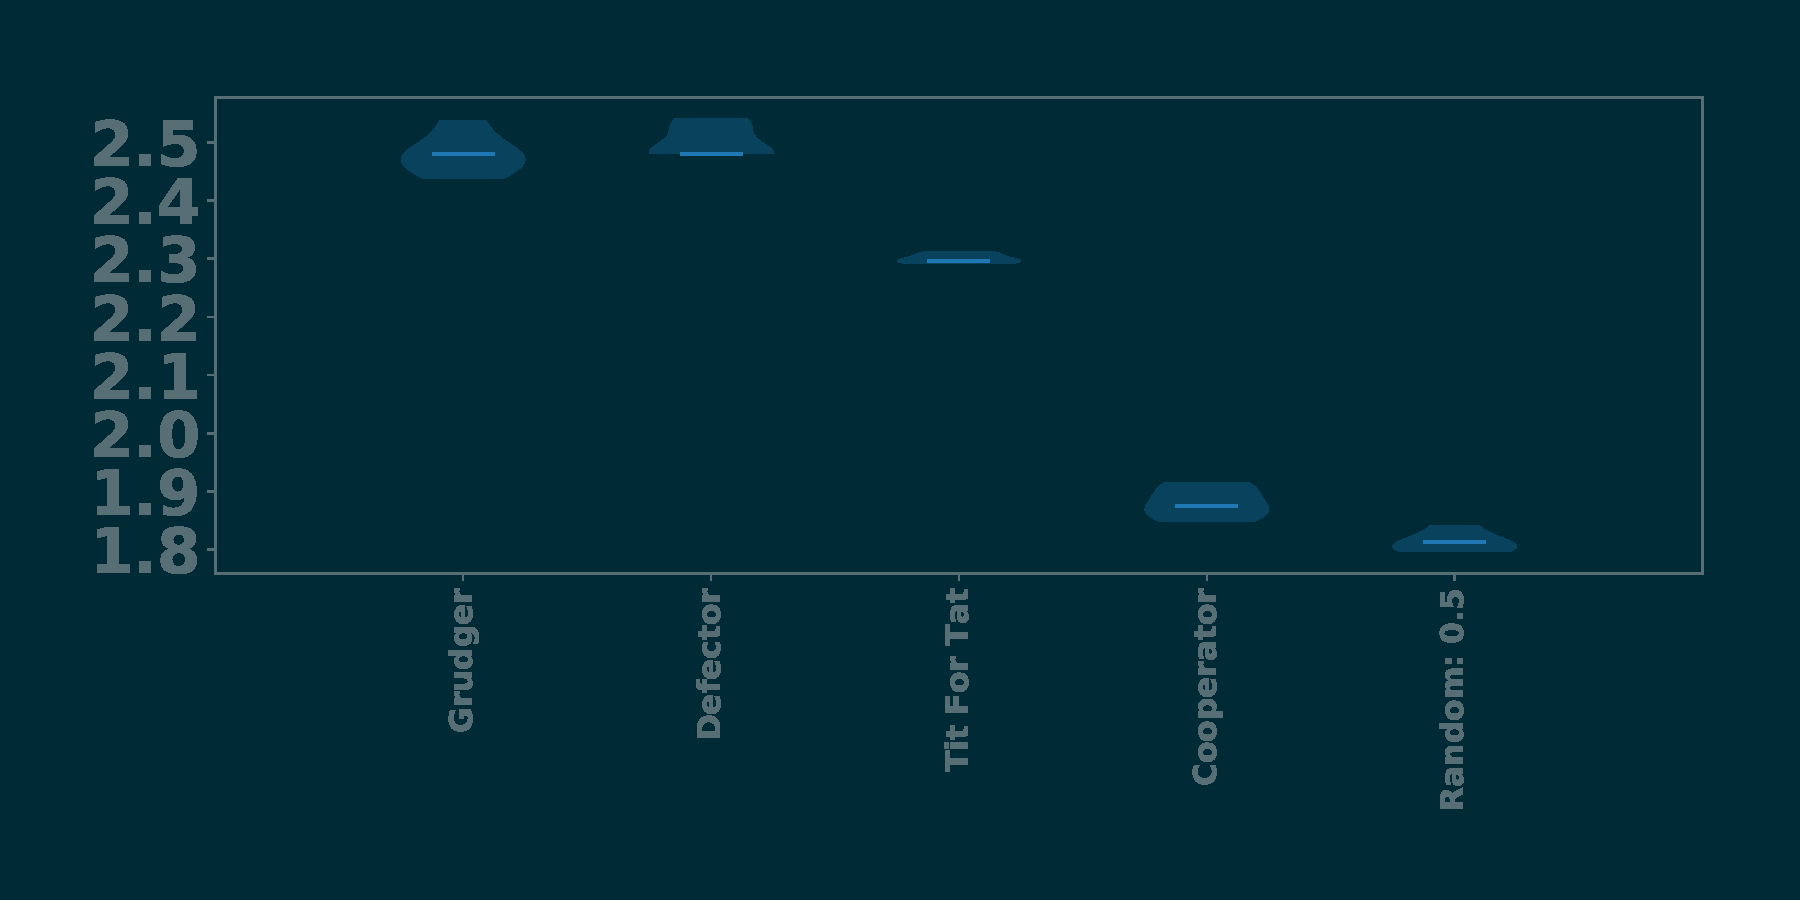
\includegraphics[width=\textwidth, height=0.65\textwidth]{static/tournament_results.pdf}
  \end{column}
      \begin{column}{.25\linewidth}
%%%%%%%%%%%%%%%%%%THIRD QUESTION%%%%%%%%%%%%%%%%%%
   \vspace{1cm}

\begin{center}
        \Large{\textcolor{cyan}{SHOULD THE NORTH JOIN HANDS WITH THE SOUTH TO DEFEAT THE NIGHT KING?}}
\end{center}

   \vspace{1.2cm}

        \begin{center}
        \includestandalone[width=1.1\textwidth]{static/evolution}
        \end{center}
    \begin{center}

    \begin{minted}
    [
    autogobble=true,
    framesep=2mm,
    fontsize=\small,
    bgcolor=DarkGray,
    ]
    {python}
>>> import axelrod as axl
>>> import random

>>> N = 5
>>> players = []
>>> axl.seed(5)
>>> for _ in range(N):
...     player = random.choice([axl.Defector,
...                             axl.Cooperator])
...     players.append(player())

>>> mp = axl.MoranProcess(players=players, turns=200)
>>> mp.play()
[Counter({'Cooperator': 3, 'Defector': 2}),
 Counter({'Cooperator': 3, 'Defector': 2}),
 Counter({'Cooperator': 3, 'Defector': 2}),
 Counter({'Cooperator': 2, 'Defector': 3}),
 Counter({'Cooperator': 2, 'Defector': 3}),
 Counter({'Cooperator': 1, 'Defector': 4}),
 Counter({'Cooperator': 1, 'Defector': 4}),
 Counter({'Cooperator': 1, 'Defector': 4}),
 Counter({'Defector': 5})]

    \end{minted}

   \vspace{1cm}

    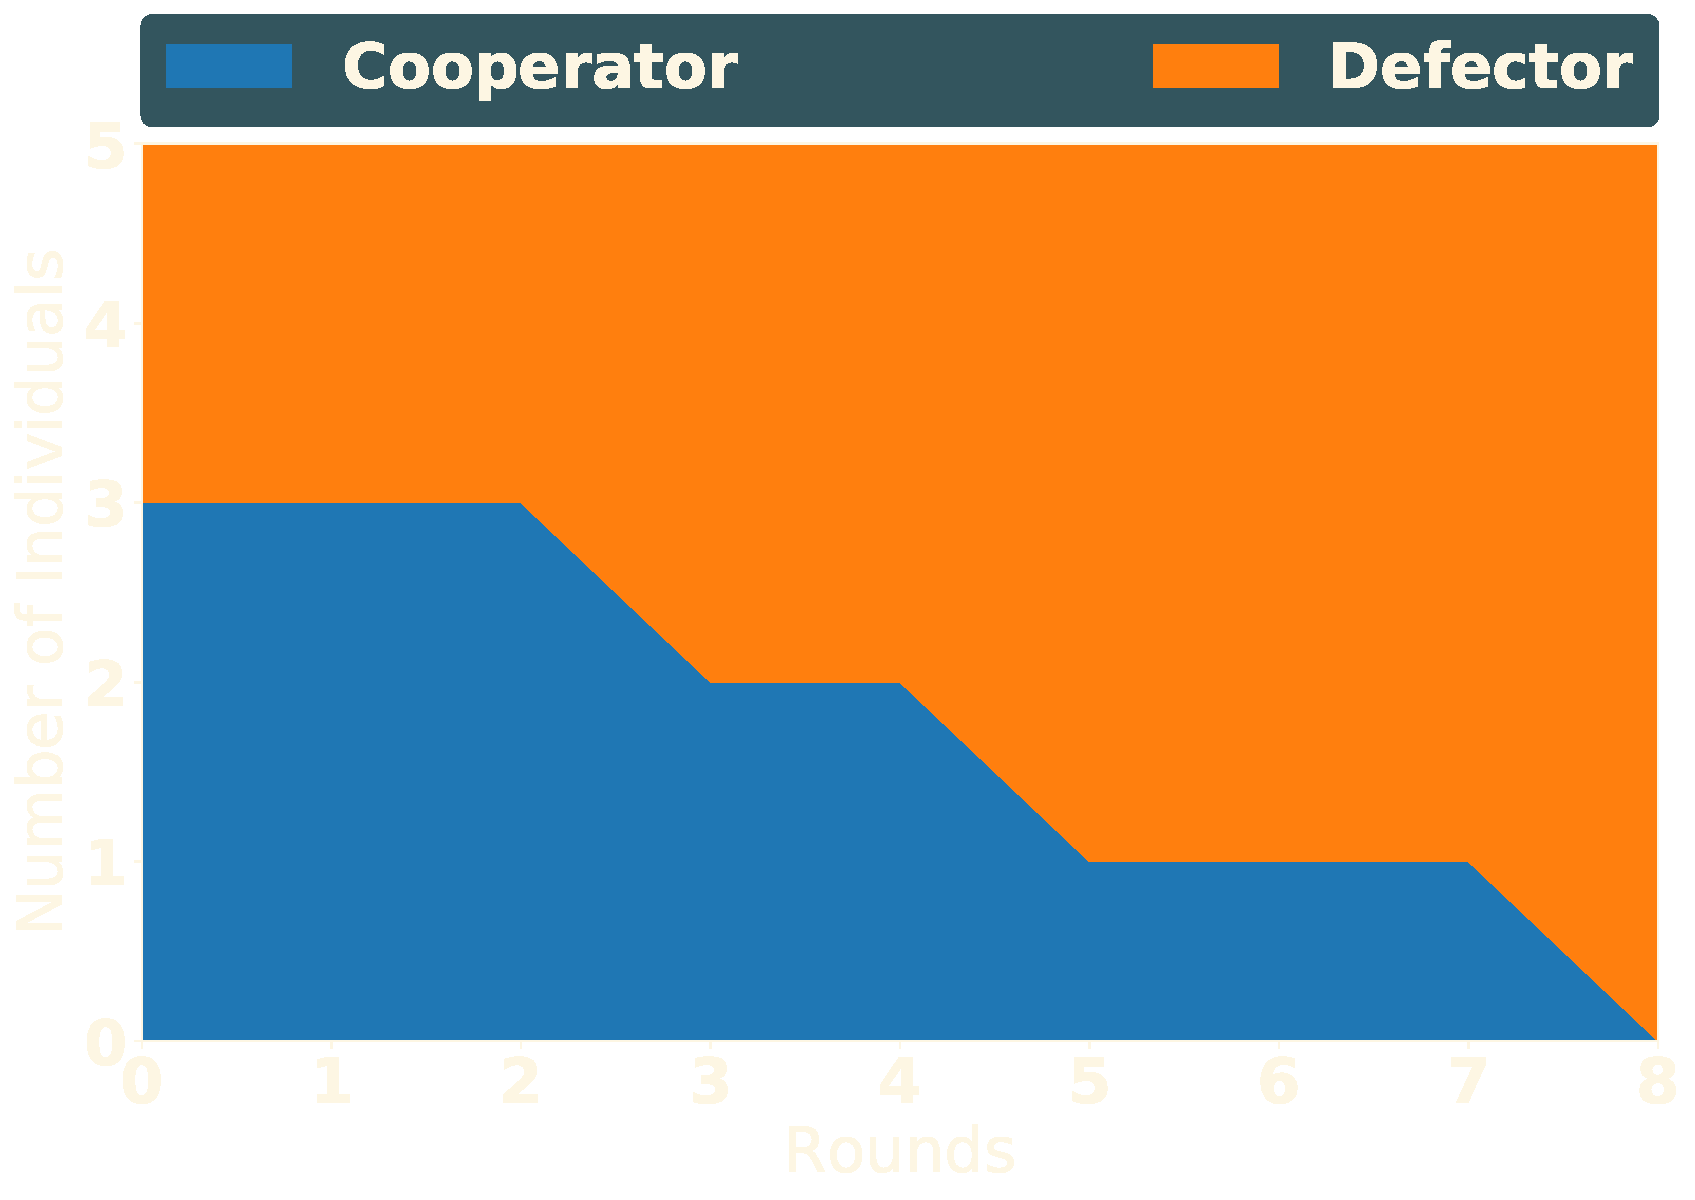
\includegraphics[width=0.8\textwidth, height=0.5\textwidth]{static/evolution_results.pdf}
    \end{center}

    \end{column}
    \end{columns}
\begin{columns}
\begin{column}{.15\linewidth}
\end{column}
\begin{column}{.8\linewidth}

   \hspace{1cm}

\textbf{ \faTwitter \ NikoletaGlyn \hspace{2cm} In case you missed me: \url{nikoleta-v3.github.io/blog/2017/08/23/grudges-war-GoT.html} \hspace{2cm} \faGithub \ Nikoleta-v3}

\end{column}
% \begin{column}{.1\linewidth}
% \end{column}
\end{columns}

   \vspace{1cm}

\end{frame}
\end{document}
